\chapter{Resultados e Discussão}
\label{cap:resultados}

Este capítulo apresenta os resultados da aplicação do artefato aos microdados das edições de 2019, 2020 e 2021 do ENEM. Conforme o protocolo da Seção~\ref{sec:auditoria}, \textbf{todas as métricas foram calculadas exclusivamente sobre o conjunto de teste} de cada edição ($n = 10.000$). As tabelas deste capítulo são geradas automaticamente a partir dos arquivos Parquet produzidos pelo pipeline\footnote{Script \texttt{article/scripts/gerar\_resultados.py}. A reexecução do pipeline seguida desse script reproduz integralmente as tabelas e figuras.}, o que assegura a correspondência exata entre o texto e os artefatos computacionais.

% ---------------------------------------------------------------------------
\section{Desempenho do Modelo-Alvo}
\label{sec:res_desempenho}

A Tabela~\ref{tab:desempenho} apresenta o desempenho do classificador no conjunto de teste. Nas três edições, a busca em grade selecionou a mesma configuração (100 árvores, profundidade máxima 3 e taxa de aprendizado 0,1), e o desempenho manteve-se estável: acurácia entre 0,6822 e 0,6842 e AUC-ROC entre 0,7475 e 0,7511. Os três hiperparâmetros selecionados situam-se nos limites da grade (maior número de árvores, menor profundidade e maior taxa de aprendizado). Isso indica que uma grade mais ampla poderia produzir ganhos marginais de desempenho. Esse refinamento não foi perseguido porque o propósito do modelo é servir de objeto representativo para a auditoria (Seção~\ref{sec:modelo}).

% ARQUIVO GERADO AUTOMATICAMENTE por article/scripts/gerar_resultados.py
% Fonte: data/outputs/*.parquet — NÃO EDITAR À MÃO.
\begin{table}[htbp]
\centering
\caption{Desempenho do modelo-alvo (XGBoost) no conjunto de teste}
\label{tab:desempenho}
\resizebox{\textwidth}{!}{%
\begin{tabular}{lccccccc}
\toprule
\textbf{Edição} & \textbf{Acurácia} & \textbf{Precisão} & \textbf{Recall} & \textbf{F1} & \textbf{AUC-ROC} & \textbf{n\_est. / prof. / taxa} & \textbf{$n_{\text{teste}}$} \\
\midrule
2019 & 0,6842 & 0,7000 & 0,6490 & 0,6736 & 0,7511 & 100 / 3 / 0,10 & 10.000 \\
2020 & 0,6825 & 0,6926 & 0,6584 & 0,6751 & 0,7475 & 100 / 3 / 0,10 & 10.000 \\
2021 & 0,6822 & 0,6868 & 0,6673 & 0,6769 & 0,7480 & 100 / 3 / 0,10 & 10.000 \\
\bottomrule
\end{tabular}}
\fonte{Elaborado pelo autor a partir de \texttt{model\_metrics\_\{ano\}.parquet}.}
\end{table}


O desempenho é moderado, o que é esperado para um modelo que dispõe apenas de seis variáveis socioeconômicas e nenhuma informação sobre a trajetória escolar do candidato. O resultado (F1 entre 0,674 e 0,677) é inferior, mas da mesma ordem de grandeza, ao relatado por \citeonline{luz2025uso}, cujo melhor modelo obteve F1 de 0,758 e ROC-AUC de 0,816 com dados do ENEM 2023. A comparação exige duas ressalvas: aquele estudo emprega um conjunto mais amplo de variáveis, e sua classe positiva é o desempenho \textbf{abaixo} da média geral, enquanto aqui a classe positiva é a NMG igual ou superior à mediana da edição. Ressalta-se que o classificador é o \textbf{objeto} da auditoria, e não o produto do trabalho. Um modelo com AUC próxima de 0,75 seria considerado razoável em muitas aplicações práticas, e é justamente esse tipo de modelo, aparentemente aceitável, que a ferramenta deve ser capaz de examinar.

% ---------------------------------------------------------------------------
\section{Auditoria de Equidade por Raça/Cor}
\label{sec:res_raca}

A Tabela~\ref{tab:di_raca} e a Figura~\ref{fig:di_raca} apresentam as métricas de equidade por raça/cor. Em todas as edições, o grupo de referência (maior taxa de seleção) é o de candidatos brancos, e \textbf{todos os grupos não brancos apresentam Impacto Disparate inferior ao limiar de 0,8}, disparando o alerta da regra dos quatro quintos nas três edições.

% ARQUIVO GERADO AUTOMATICAMENTE por article/scripts/gerar_resultados.py
% Fonte: data/outputs/*.parquet — NÃO EDITAR À MÃO.
\begin{table}[htbp]
\centering
\caption{Impacto Disparate e Igualdade de Oportunidades por raça/cor no conjunto de teste, com intervalos de confiança de 95\%}
\label{tab:di_raca}
\resizebox{\textwidth}{!}{%
\begin{tabular}{lccccccc}
\toprule
\textbf{Grupo} & \textbf{$n$} & \textbf{$n$ ($Y=1$)} & \textbf{DI} & \textbf{IC95\% DI} & \textbf{TPR} & \textbf{IC95\% TPR} & \textbf{DI $<$ 0,8} \\
\midrule
\multicolumn{8}{l}{\textbf{ENEM 2019}} \\
\quad Branca (ref.) & 3.723 & 2.341 & 1,000 & -- & 0,801 & [0,784; 0,817] & Não \\
\quad Preta & 1.219 & 488 & 0,426 & [0,387; 0,465] & 0,469 & [0,424; 0,515] & \textbf{Sim} \\
\quad Parda & 4.581 & 1.954 & 0,495 & [0,472; 0,518] & 0,521 & [0,498; 0,542] & \textbf{Sim} \\
\quad Amarela & 225 & 106 & 0,609 & [0,517; 0,705] & 0,623 & [0,531; 0,710] & \textbf{Sim} \\
\quad Indígena & 52 & 19 & 0,252 & [0,115; 0,414] & 0,316 & [0,125; 0,545] & \textbf{Sim} \\
\quad Não declarada & 200 & 112 & 0,620 & [0,522; 0,720] & 0,580 & [0,491; 0,675] & \textbf{Sim} \\
\midrule
\multicolumn{8}{l}{\textbf{ENEM 2020}} \\
\quad Branca (ref.) & 3.793 & 2.386 & 1,000 & -- & 0,842 & [0,827; 0,856] & Não \\
\quad Preta & 1.227 & 483 & 0,365 & [0,331; 0,400] & 0,418 & [0,373; 0,460] & \textbf{Sim} \\
\quad Parda & 4.505 & 1.909 & 0,462 & [0,441; 0,484] & 0,505 & [0,483; 0,528] & \textbf{Sim} \\
\quad Amarela & 230 & 117 & 0,498 & [0,417; 0,587] & 0,496 & [0,406; 0,589] & \textbf{Sim} \\
\quad Indígena & 49 & 12 & 0,169 & [0,048; 0,310] & 0,167 & [0,000; 0,429] & \textbf{Sim} \\
\quad Não declarada & 196 & 102 & 0,633 & [0,539; 0,735] & 0,627 & [0,533; 0,726] & \textbf{Sim} \\
\midrule
\multicolumn{8}{l}{\textbf{ENEM 2021}} \\
\quad Branca (ref.) & 4.427 & 2.730 & 1,000 & -- & 0,830 & [0,816; 0,844] & Não \\
\quad Preta & 1.104 & 405 & 0,337 & [0,302; 0,373] & 0,343 & [0,298; 0,390] & \textbf{Sim} \\
\quad Parda & 4.022 & 1.643 & 0,423 & [0,401; 0,444] & 0,477 & [0,453; 0,501] & \textbf{Sim} \\
\quad Amarela & 211 & 109 & 0,663 & [0,570; 0,759] & 0,706 & [0,617; 0,792] & \textbf{Sim} \\
\quad Indígena & 47 & 9 & 0,417 & [0,231; 0,613] & 0,778 & [0,429; 1,000] & \textbf{Sim} \\
\quad Não declarada & 189 & 93 & 0,629 & [0,530; 0,731] & 0,602 & [0,500; 0,703] & \textbf{Sim} \\
\bottomrule
\end{tabular}}
\fonte{Elaborado pelo autor a partir de \texttt{fairness\_metrics\_\{ano\}.parquet}. Grupo de referência: maior taxa de seleção. IC95\%: percentis 2,5 e 97,5 de 2.000 reamostragens \textit{bootstrap} do conjunto de teste, com o modelo fixo. A FPR por grupo é apresentada na Figura~\ref{fig:tpr_fpr}.}
\end{table}


\begin{figure}[htbp]
\centering
\caption{Impacto Disparate por raça/cor no conjunto de teste}
\label{fig:di_raca}
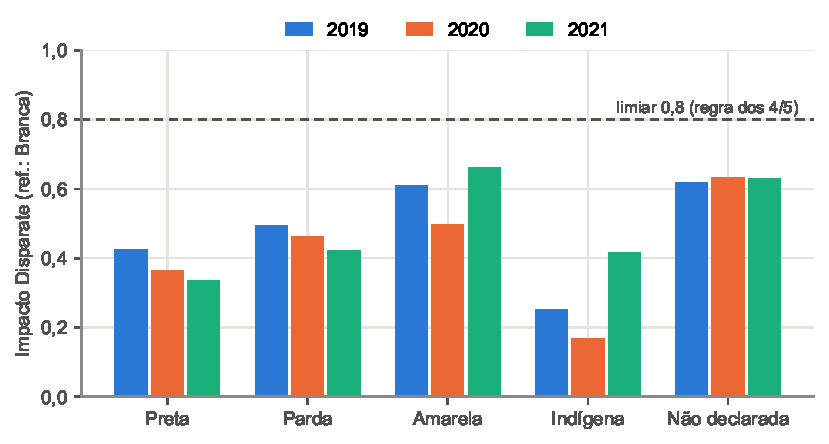
\includegraphics[width=\textwidth]{figuras/resultados/fig_di_raca.pdf}
\fonte{Elaborado pelo autor a partir de \texttt{fairness\_metrics\_\{ano\}.parquet}.}
\end{figure}

Os grupos Preto e Pardo, que juntos representam mais da metade dos candidatos, apresentam as disparidades mais consistentes e com tendência de agravamento ao longo do período. O DI do grupo Preto passa de 0,426 em 2019 para 0,365 em 2020 e 0,337 em 2021; o do grupo Pardo, de 0,495 para 0,462 e 0,423. Em 2021, portanto, um candidato preto tinha cerca de um terço da probabilidade de um candidato branco de ser classificado acima da mediana.

O grupo Indígena apresenta os menores valores em 2019 (0,252) e 2020 (0,169). Esses valores, contudo, devem ser interpretados com cautela: o grupo conta com apenas 47 a 52 candidatos no conjunto de teste, e a variação abrupta observada em 2021 (0,417) é compatível com flutuação amostral (ver Seção~\ref{sec:res_limitacoes}).

Os intervalos de confiança da Tabela~\ref{tab:di_raca} permitem separar as conclusões robustas das frágeis.

O \textbf{alerta da regra dos quatro quintos é estatisticamente robusto para todos os grupos não brancos}, inclusive o Indígena. O limite superior do IC95\% do DI não ultrapassa 0,759 em nenhum caso, e em ao menos 99,5\% das reamostragens o DI permaneceu abaixo de 0,8. A tendência de agravamento dos grupos Preto e Pardo também é sustentada pelos dados: os intervalos de 2019 e 2021 não se sobrepõem (Preto: [0,387; 0,465] e [0,302; 0,373]; Pardo: [0,472; 0,518] e [0,401; 0,444]).

Em contrapartida, \textbf{as estimativas de TPR do grupo Indígena não são conclusivas}. Com apenas 19, 12 e 9 candidatos de rótulo positivo no teste, os intervalos são muito amplos ([0,000; 0,429] em 2020 e [0,429; 1,000] em 2021), e a TPR de 0,778 observada em 2021 não deve ser interpretada como evidência de igualdade de oportunidades para esse grupo.

\subsection{Igualdade de Oportunidades}

A Figura~\ref{fig:tpr_fpr} decompõe as predições segundo os rótulos reais. A disparidade não decorre apenas de diferenças nas taxas-base, pois o modelo também \textbf{erra de forma assimétrica}. Entre os candidatos que efetivamente obtiveram NMG igual ou superior à mediana, o modelo reconhece entre 80,1\% e 84,2\% dos brancos (TPR), mas apenas 46,9\%, 41,8\% e 34,3\% dos pretos em 2019, 2020 e 2021, e entre 47,7\% e 52,1\% dos pardos. Simetricamente, a FPR de candidatos brancos (0,492 a 0,530) é cerca de três vezes a de pretos (0,165 a 0,182). O modelo, portanto, concede mais ``aprovações'' indevidas ao grupo privilegiado e nega mais aprovações merecidas aos grupos protegidos, violando simultaneamente os critérios de \textit{Equal Opportunity} e \textit{Equalized Odds} \cite{hardt2016equality}.

\begin{figure}[htbp]
\centering
\caption{Taxas de verdadeiros positivos (TPR) e de falsos positivos (FPR) por raça/cor}
\label{fig:tpr_fpr}
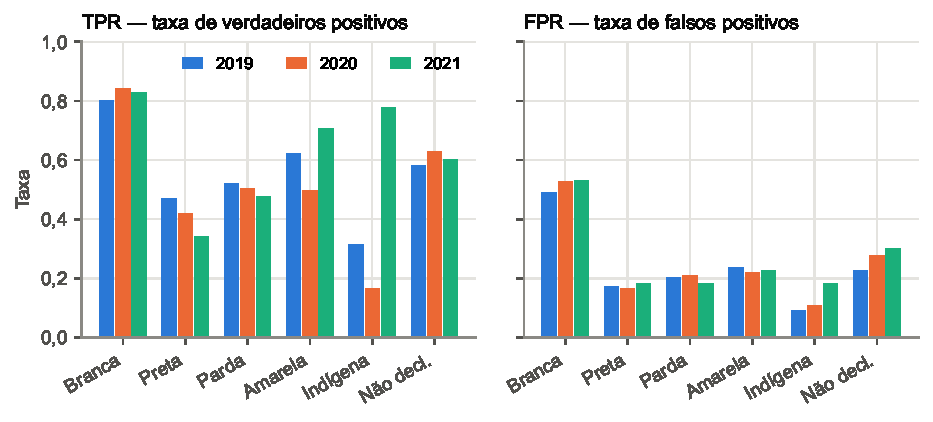
\includegraphics[width=\textwidth]{figuras/resultados/fig_tpr_fpr_raca.pdf}
\fonte{Elaborado pelo autor a partir de \texttt{fairness\_metrics\_\{ano\}.parquet}.}
\end{figure}

% ---------------------------------------------------------------------------
\section{Auditoria de Equidade por Renda Familiar}
\label{sec:res_renda}

A renda familiar produz o gradiente de disparidade mais acentuado (Tabela~\ref{tab:di_renda} e Figura~\ref{fig:di_renda}). Nas três edições, \textbf{as faixas A a E (renda familiar de até 2,5 salários mínimos) violam a regra dos quatro quintos}, e as faixas A e B (nenhuma renda e até 1 salário mínimo) apresentam DI entre 0,044 e 0,074, de modo que o modelo praticamente nunca classifica esses candidatos acima da mediana. A desigualdade de oportunidades é igualmente extrema: na faixa B, a TPR é de apenas 0,077 em 2019, 0,126 em 2020 e 0,115 em 2021, ou seja, quase nove em cada dez candidatos de baixa renda que superaram a mediana são classificados incorretamente.

% ARQUIVO GERADO AUTOMATICAMENTE por article/scripts/gerar_resultados.py
% Fonte: data/outputs/*.parquet — NÃO EDITAR À MÃO.
\begin{table}[htbp]
\centering
\caption{Impacto Disparate e TPR por faixa de renda familiar (Q006) no conjunto de teste}
\label{tab:di_renda}
\begin{tabular}{llcccccc}
\toprule
 & & \multicolumn{3}{c}{\textbf{DI}} & \multicolumn{3}{c}{\textbf{TPR}} \\
\cmidrule(lr){3-5}\cmidrule(lr){6-8}
\textbf{Faixa} & \textbf{Renda mensal} & 2019 & 2020 & 2021 & 2019 & 2020 & 2021 \\
\midrule
A & Nenhuma renda & \textbf{0,070} & \textbf{0,072} & \textbf{0,044} & 0,190 & 0,181 & 0,108 \\
B & Até 1 SM & \textbf{0,047} & \textbf{0,074} & \textbf{0,053} & 0,077 & 0,126 & 0,115 \\
C & 1 a 1,5 SM & \textbf{0,209} & \textbf{0,356} & \textbf{0,207} & 0,284 & 0,447 & 0,290 \\
D & 1,5 a 2 SM & \textbf{0,662} & \textbf{0,569} & \textbf{0,481} & 0,736 & 0,664 & 0,575 \\
E & 2 a 2,5 SM & \textbf{0,771} & \textbf{0,764} & \textbf{0,723} & 0,858 & 0,827 & 0,767 \\
F & 2,5 a 3 SM & 0,848 & 0,855 & 0,803 & 0,884 & 0,883 & 0,869 \\
G & 3 a 4 SM & 0,897 & 0,947 & 0,883 & 0,921 & 0,961 & 0,911 \\
H & 4 a 5 SM & 0,976 & 0,982 & 0,938 & 0,983 & 0,989 & 0,961 \\
I & 5 a 6 SM & 0,968 & 0,983 & 0,974 & 0,981 & 0,984 & 0,973 \\
J & 6 a 7 SM & 0,995 & 1,000 & 0,990 & 0,994 & 1,000 & 0,987 \\
K & 7 a 8 SM & 0,986 & 0,992 & 0,981 & 1,000 & 1,000 & 0,991 \\
L & 8 a 9 SM & 1,000 & 1,000 & 1,000 & 1,000 & 1,000 & 1,000 \\
M & 9 a 10 SM & 0,989 & 1,000 & 0,986 & 0,987 & 1,000 & 0,988 \\
N & 10 a 12 SM & 1,000 & 1,000 & 0,993 & 1,000 & 1,000 & 0,991 \\
O & 12 a 15 SM & 0,990 & 1,000 & 0,992 & 1,000 & 1,000 & 0,991 \\
P & 15 a 20 SM & 1,000 & 0,991 & 0,985 & 1,000 & 1,000 & 0,991 \\
Q & Acima de 20 SM & 1,000 & 1,000 & 1,000 & 1,000 & 1,000 & 1,000 \\
\bottomrule
\end{tabular}
\fonte{Elaborado pelo autor a partir de \texttt{fairness\_metrics\_\{ano\}.parquet}. SM = salário mínimo vigente no ano. Em negrito: DI $<$ 0,8. Faixa de referência (maior taxa de seleção) --- 2019: L, 2020: J, 2021: L.}
\end{table}


\begin{figure}[htbp]
\centering
\caption{Impacto Disparate por faixa de renda familiar (Q006)}
\label{fig:di_renda}
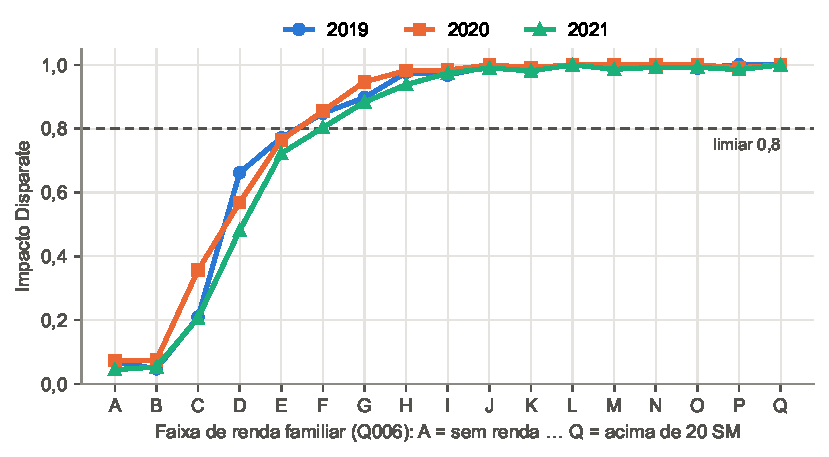
\includegraphics[width=\textwidth]{figuras/resultados/fig_di_renda.pdf}
\fonte{Elaborado pelo autor a partir de \texttt{fairness\_metrics\_\{ano\}.parquet}.}
\end{figure}

A fronteira do alerta situa-se entre as faixas E e F. Na faixa E, o DI fica abaixo de 0,8 em pelo menos 98\% das reamostragens \textit{bootstrap} nas três edições. Já a faixa F em 2021 ($\mathrm{DI} = 0{,}803$, com IC95\% de [0,774; 0,832]) encontra-se sobre o limiar: o DI ficou abaixo de 0,8 em 41,2\% das reamostragens, e a ausência de alerta nesse caso não deve ser lida como conformidade. A partir da faixa F, o DI aproxima-se de 1, e diversas faixas superiores empatam com taxas de seleção próximas de 100\%. Por esse motivo, o grupo de referência varia entre as edições (faixas L, J e L), sem impacto relevante sobre os valores de DI das faixas inferiores. Como os limites das faixas são expressos em salários mínimos vigentes em cada ano, a comparação entre edições deve ser entendida em termos relativos.

% ---------------------------------------------------------------------------
\section{Amplificação do Viés pelo Modelo}
\label{sec:res_amplificacao}

Uma questão central para a auditoria é se o modelo apenas \textbf{reproduz} a desigualdade presente nos dados ou se a \textbf{amplifica}. A Tabela~\ref{tab:amplificacao} e a Figura~\ref{fig:amplificacao} comparam o DI calculado sobre os rótulos reais ($\mathrm{DI}_y$) com o DI das predições ($\mathrm{DI}_{\hat{y}}$), conforme a Equação~\eqref{eq:amplificacao}.

% ARQUIVO GERADO AUTOMATICAMENTE por article/scripts/gerar_resultados.py
% Fonte: data/outputs/*.parquet — NÃO EDITAR À MÃO.
\begin{table}[htbp]
\centering
\caption{Impacto Disparate dos rótulos reais ($y$) versus das predições ($\hat{y}$) por raça/cor}
\label{tab:amplificacao}
\resizebox{\textwidth}{!}{%
\begin{tabular}{l*{9}{c}}
\toprule
 & \multicolumn{3}{c}{\textbf{2019}} & \multicolumn{3}{c}{\textbf{2020}} & \multicolumn{3}{c}{\textbf{2021}} \\
\cmidrule(lr){2-4}\cmidrule(lr){5-7}\cmidrule(lr){8-10}
\textbf{Grupo} & $\mathrm{DI}_y$ & $\mathrm{DI}_{\hat{y}}$ & $\Delta$ & $\mathrm{DI}_y$ & $\mathrm{DI}_{\hat{y}}$ & $\Delta$ & $\mathrm{DI}_y$ & $\mathrm{DI}_{\hat{y}}$ & $\Delta$ \\
\midrule
Preta & 0,637 & 0,426 & −0,211 & 0,626 & 0,365 & −0,260 & 0,595 & 0,337 & −0,258 \\
Parda & 0,678 & 0,495 & −0,183 & 0,674 & 0,462 & −0,212 & 0,662 & 0,423 & −0,240 \\
Amarela & 0,749 & 0,609 & −0,140 & 0,809 & 0,498 & −0,311 & 0,838 & 0,663 & −0,175 \\
Indígena & 0,581 & 0,252 & −0,329 & 0,389 & 0,169 & −0,220 & 0,311 & 0,417 & +0,106 \\
Não declarada & 0,891 & 0,620 & −0,271 & 0,827 & 0,633 & −0,194 & 0,798 & 0,629 & −0,169 \\
\bottomrule
\end{tabular}}
\fonte{Elaborado pelo autor a partir de \texttt{fairness\_metrics\_\{ano\}.parquet}. Referência: Branca. $\Delta = \mathrm{DI}_{\hat{y}} - \mathrm{DI}_y$ (valores negativos indicam amplificação da disparidade pelo modelo).}
\end{table}


\begin{figure}[htbp]
\centering
\caption{Impacto Disparate dos rótulos reais e das predições, por raça/cor}
\label{fig:amplificacao}
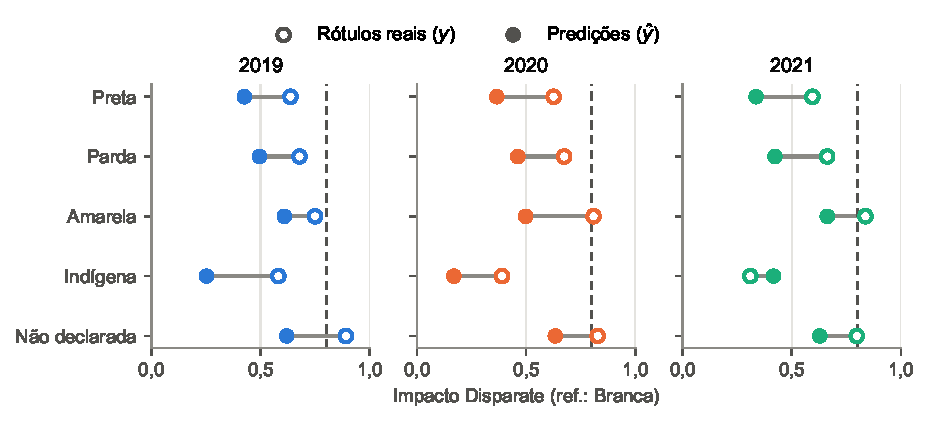
\includegraphics[width=\textwidth]{figuras/resultados/fig_amplificacao.pdf}
\fonte{Elaborado pelo autor a partir de \texttt{fairness\_metrics\_\{ano\}.parquet}.}
\end{figure}

Em 14 das 15 combinações de grupo e edição, o DI das predições é inferior ao dos rótulos, com reduções entre 0,140 e 0,329. O caso mais revelador é o de grupos que \textbf{satisfazem a regra dos quatro quintos nos dados, mas passam a violá-la no modelo}: candidatos que não declararam raça/cor em 2019 (DI\textsubscript{$y$} = 0,891 → DI\textsubscript{$\hat{y}$} = 0,620) e em 2020 (0,827 → 0,633), e candidatos amarelos em 2020 (0,809 → 0,498) e em 2021 (0,838 → 0,663). Nesses casos, a disparidade que dispara o alerta é \textbf{introduzida} pelo classificador, e não herdada dos rótulos.

O mecanismo é inerente a classificadores com limiar de decisão. Quando a maior parte dos perfis socioeconômicos de um grupo tem probabilidade estimada inferior a 0,5, o modelo atribui a classe negativa a quase todos os seus membros, comprimindo a taxa de seleção abaixo da taxa-base real. A única exceção (Indígena, 2021, $\Delta$ = +0,106) ocorre no grupo com apenas 47 candidatos no teste.

% ---------------------------------------------------------------------------
\section{Explicabilidade: Fatores Determinantes das Predições}
\label{sec:res_shap}

A Tabela~\ref{tab:shap} apresenta o ranking de importância global SHAP (Equação~\eqref{eq:importancia}) e a Figura~\ref{fig:shap} compara a importância dos principais atributos entre as edições.

% ARQUIVO GERADO AUTOMATICAMENTE por article/scripts/gerar_resultados.py
% Fonte: data/outputs/*.parquet — NÃO EDITAR À MÃO.
\begin{table}[htbp]
\centering
\caption{Ranking de importância global SHAP (média de $|\phi_i|$, escala log-odds) no conjunto de teste}
\label{tab:shap}
\resizebox{\textwidth}{!}{%
\begin{tabular}{clclclc}
\toprule
 & \multicolumn{2}{c}{\textbf{2019}} & \multicolumn{2}{c}{\textbf{2020}} & \multicolumn{2}{c}{\textbf{2021}} \\
\cmidrule(lr){2-3}\cmidrule(lr){4-5}\cmidrule(lr){6-7}
\textbf{\#} & \textbf{Atributo} & $\overline{|\phi|}$ & \textbf{Atributo} & $\overline{|\phi|}$ & \textbf{Atributo} & $\overline{|\phi|}$ \\
\midrule
1 & Computador: nenhum computador & 0,405 & Computador: nenhum computador & 0,448 & Computador: nenhum computador & 0,506 \\
2 & Renda: até 1 SM & 0,186 & Renda: até 1 SM & 0,194 & Computador: um computador & 0,203 \\
3 & Renda: 1 a 1,5 SM & 0,134 & Raça/cor: branca & 0,164 & Renda: até 1 SM & 0,181 \\
4 & Raça/cor: branca & 0,130 & Computador: um computador & 0,137 & Raça/cor: branca & 0,148 \\
5 & Computador: um computador & 0,095 & Renda: 1 a 1,5 SM & 0,085 & Renda: 1 a 1,5 SM & 0,082 \\
6 & Escol. da mãe: superior completo & 0,083 & Renda: nenhuma renda & 0,075 & Escol. do pai: superior completo & 0,077 \\
7 & Escol. da mãe: médio completo & 0,081 & Escol. do pai: médio completo & 0,071 & Escol. do pai: médio completo & 0,073 \\
8 & Escol. da mãe: pós-graduação & 0,075 & Escol. da mãe: médio completo & 0,068 & Renda: nenhuma renda & 0,065 \\
\bottomrule
\end{tabular}}
\fonte{Elaborado pelo autor a partir de \texttt{shap\_values\_\{ano\}.parquet}.}
\end{table}


\begin{figure}[htbp]
\centering
\caption{Importância global SHAP dos principais atributos, por edição}
\label{fig:shap}
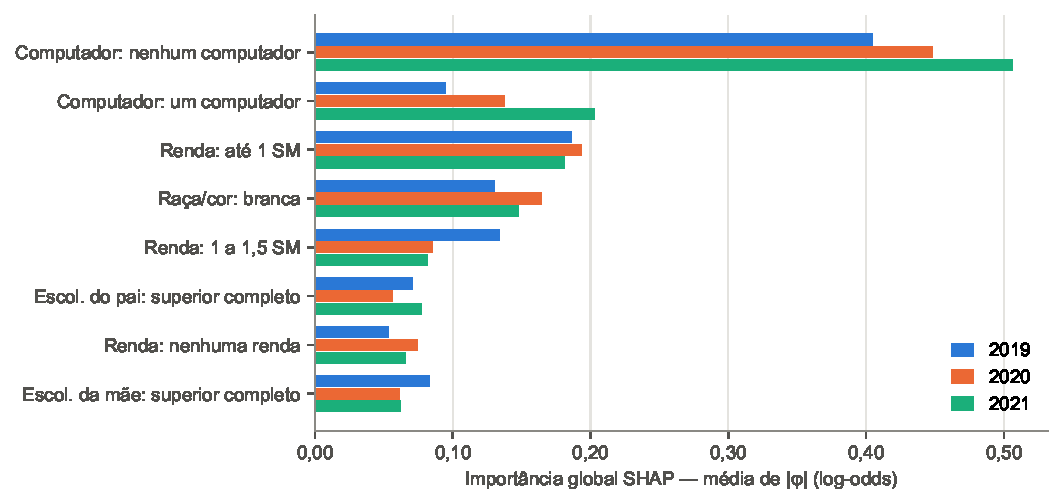
\includegraphics[width=\textwidth]{figuras/resultados/fig_shap_global.pdf}
\fonte{Elaborado pelo autor a partir de \texttt{shap\_values\_\{ano\}.parquet}.}
\end{figure}

Três achados se destacam. Primeiro, \textbf{a ausência de computador na residência (Q024 = A) é o atributo de maior influência nas três edições}, e seu peso cresce continuamente: a importância média passa de 0,405 em 2019 para 0,448 em 2020 e 0,506 em 2021, um aumento de 25\%. A categoria ``um computador'' segue a mesma tendência, saltando da quinta posição (0,095) em 2019 para a segunda (0,203) em 2021. O crescimento é temporalmente coincidente com o período de ensino remoto emergencial da pandemia de COVID-19, em que o acesso a equipamentos digitais tornou-se condição para a continuidade dos estudos. O resultado é \textbf{compatível} com a hipótese de agravamento da exclusão digital, mas o desenho do estudo, que é observacional e sem grupo de comparação, \textbf{não permite atribuí-lo causalmente à pandemia}. Ressalva-se, ainda, que os valores SHAP descrevem o comportamento do modelo, e não relações causais, e que a composição dos participantes mudou entre as edições (de 3,70 milhões de presentes em 2019 para 2,24 milhões em 2021), o que também pode contribuir para o efeito.

Uma objeção técnica a essa comparação é que a importância média $\overline{|\phi|}$ de uma variável indicadora depende não apenas do efeito da categoria, mas também de sua \textbf{prevalência}. O aumento poderia, portanto, refletir apenas uma mudança na proporção de candidatos sem computador. A Tabela~\ref{tab:shap_q024} descarta essa explicação. A prevalência de candidatos sem computador no teste \textbf{diminuiu} de 0,445 em 2019 para 0,381 em 2021. No mesmo período, a diferença entre a contribuição SHAP média de quem possui e de quem não possui computador \textbf{aumentou} de 0,830 para 1,116 log-odds, um crescimento de 34\%. O peso atribuído pelo modelo à ausência de computador cresceu, portanto, por candidato, e não por efeito de composição. A queda da prevalência em 2021 é, por sua vez, coerente com a redução do número de participantes e com a hipótese de que candidatos mais vulneráveis deixaram de realizar o exame.

% ARQUIVO GERADO AUTOMATICAMENTE por article/scripts/gerar_resultados.py
% Fonte: data/outputs/*.parquet — NÃO EDITAR À MÃO.
\begin{table}[htbp]
\centering
\caption{Decomposição da importância SHAP do atributo ``sem computador'' (Q024 = A) por edição}
\label{tab:shap_q024}
\begin{tabular}{cccccc}
\toprule
\textbf{Edição} & \textbf{Prevalência} & $\overline{|\phi|}$ & $\bar{\phi}$ \textbf{(sem comp.)} & $\bar{\phi}$ \textbf{(com comp.)} & \textbf{Diferença} \\
\midrule
2019 & 0,445 & 0,405 & −0,505 & 0,325 & 0,830 \\
2020 & 0,444 & 0,448 & −0,564 & 0,356 & 0,920 \\
2021 & 0,381 & 0,506 & −0,774 & 0,342 & 1,116 \\
\bottomrule
\end{tabular}
\fonte{Elaborado pelo autor a partir de \texttt{shap\_feature\_summary\_\{ano\}.parquet}. Prevalência: proporção de candidatos sem computador no teste. Diferença: $\bar{\phi}$ (com comp.) $-$ $\bar{\phi}$ (sem comp.), em log-odds.}
\end{table}


Segundo, \textbf{a renda familiar mais baixa} (até 1 salário mínimo) mantém-se entre os três atributos mais relevantes em todas as edições, ao lado das demais faixas inferiores de renda e da escolaridade dos pais, em consonância com a literatura sobre o peso do capital econômico e cultural familiar no desempenho \cite{souza2025desigualdades}.

Terceiro, \textbf{a raça/cor branca figura entre os quatro atributos mais importantes em todas as edições} (4.ª posição em 2019 e 2021; 3.ª em 2020). Mesmo dispondo de renda, escolaridade dos pais e acesso a tecnologia, o modelo utiliza diretamente a raça/cor como sinal preditivo. Essa constatação, que as métricas de equidade sozinhas não permitiriam estabelecer, ilustra o valor da camada de explicabilidade para localizar a \textbf{origem} das disparidades.

% ---------------------------------------------------------------------------
\section{Validação por Injeção Sintética de Viés}
\label{sec:res_injecao}

Esta seção apresenta a avaliação do artefato pelo experimento controlado descrito na Seção~\ref{sec:injecao}. A Tabela~\ref{tab:injecao} e a Figura~\ref{fig:injecao} mostram, para cada intensidade de injeção, o DI médio do grupo-alvo nos cenários de injeção direcionada e de controle negativo, bem como a AUC-ROC do modelo retreinado.

% ARQUIVO GERADO AUTOMATICAMENTE por article/scripts/gerar_resultados.py
% Fonte: data/outputs/*.parquet — NÃO EDITAR À MÃO.
\begin{table}[htbp]
\centering
\caption{Curva de sensibilidade: DI médio do grupo-alvo e AUC-ROC sob injeção sintética de viés (teste)}
\label{tab:injecao}
\resizebox{\textwidth}{!}{%
\begin{tabular}{l*{9}{c}}
\toprule
 & \multicolumn{3}{c}{\textbf{2019}} & \multicolumn{3}{c}{\textbf{2020}} & \multicolumn{3}{c}{\textbf{2021}} \\
\cmidrule(lr){2-4}\cmidrule(lr){5-7}\cmidrule(lr){8-10}
\textbf{Intensidade $p$} & DI (injeção) & DI (controle) & AUC & DI (injeção) & DI (controle) & AUC & DI (injeção) & DI (controle) & AUC \\
\midrule
\multicolumn{10}{l}{\textbf{Grupo-alvo: Parda}} \\
\quad 0\% & 0,495 $\pm$ 0,000 & 0,495 & 0,751 & 0,462 $\pm$ 0,000 & 0,462 & 0,748 & 0,423 $\pm$ 0,000 & 0,423 & 0,748 \\
\quad 10\% & 0,384 $\pm$ 0,006 & 0,448 & 0,750 & 0,372 $\pm$ 0,007 & 0,434 & 0,746 & 0,344 $\pm$ 0,014 & 0,421 & 0,747 \\
\quad 25\% & 0,189 $\pm$ 0,011 & 0,432 & 0,743 & 0,184 $\pm$ 0,004 & 0,412 & 0,739 & 0,165 $\pm$ 0,001 & 0,405 & 0,740 \\
\quad 50\% & 0,005 $\pm$ 0,002 & 0,325 & 0,719 & 0,008 $\pm$ 0,005 & 0,318 & 0,717 & 0,005 $\pm$ 0,003 & 0,302 & 0,721 \\
\midrule
\multicolumn{10}{l}{\textbf{Grupo-alvo: Indígena}} \\
\quad 0\% & 0,252 $\pm$ 0,000 & 0,252 & 0,751 & 0,169 $\pm$ 0,000 & 0,169 & 0,748 & 0,417 $\pm$ 0,000 & 0,417 & 0,748 \\
\quad 10\% & 0,207 $\pm$ 0,015 & 0,257 & 0,751 & 0,152 $\pm$ 0,025 & 0,197 & 0,748 & 0,380 $\pm$ 0,013 & 0,419 & 0,748 \\
\quad 25\% & 0,190 $\pm$ 0,024 & 0,257 & 0,751 & 0,118 $\pm$ 0,012 & 0,186 & 0,748 & 0,250 $\pm$ 0,054 & 0,419 & 0,748 \\
\quad 50\% & 0,072 $\pm$ 0,015 & 0,256 & 0,751 & 0,079 $\pm$ 0,024 & 0,197 & 0,748 & 0,066 $\pm$ 0,039 & 0,417 & 0,748 \\
\bottomrule
\end{tabular}}
\fonte{Elaborado pelo autor a partir de \texttt{bias\_injection\_summary.parquet}. Média $\pm$ desvio-padrão de 5 repetições. AUC do cenário de injeção.}
\end{table}


\begin{figure}[htbp]
\centering
\caption{Curva de sensibilidade: DI do grupo-alvo (acima) e AUC-ROC (abaixo) em função da intensidade de injeção}
\label{fig:injecao}
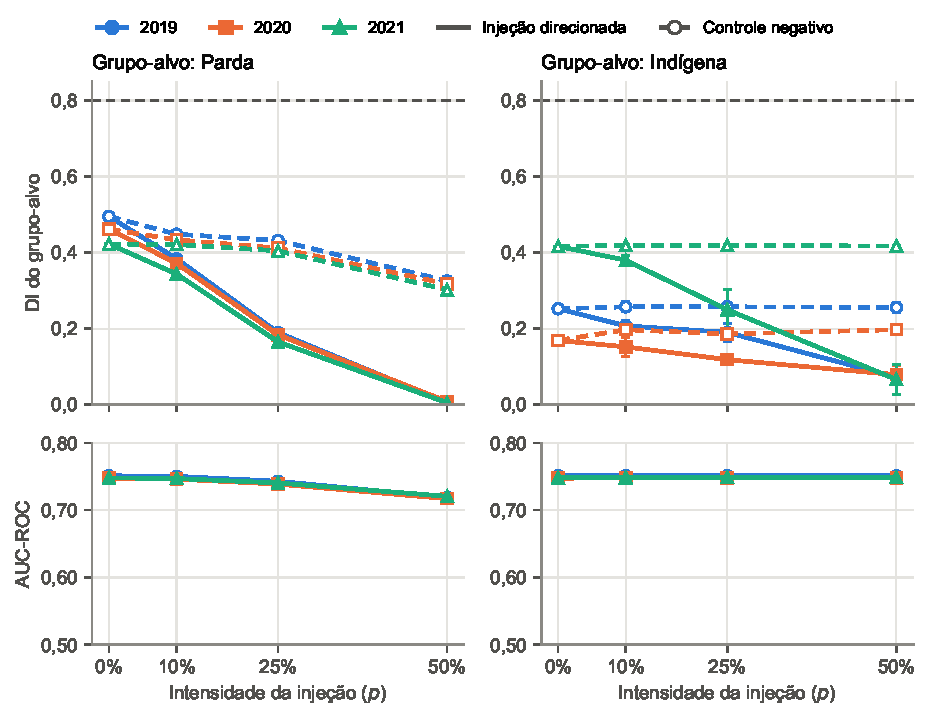
\includegraphics[width=\textwidth]{figuras/resultados/fig_injecao.pdf}
\fonte{Elaborado pelo autor a partir de \texttt{bias\_injection\_summary.parquet}. Barras: $\pm$ 1 desvio-padrão (5 repetições).}
\end{figure}

\subsection{Sensibilidade (H1)}

A hipótese H1 é confirmada em todas as seis combinações de grupo e edição: o DI médio decresce estritamente a cada aumento da intensidade de injeção. Para o grupo Pardo, o DI cai de 0,495 para 0,005 em 2019, de 0,462 para 0,008 em 2020 e de 0,423 para 0,005 em 2021 com 50\% de injeção, ou seja, o modelo deixa de selecionar praticamente qualquer candidato pardo. Para o grupo Indígena, a queda é de 0,252 para 0,072, de 0,169 para 0,079 e de 0,417 para 0,066. A baixa variabilidade entre repetições no grupo Pardo (desvio-padrão máximo de 0,014) indica que o indicador responde de forma estável à magnitude do viés.

\subsection{Especificidade (H2)}

No grupo Indígena, o controle negativo praticamente não altera o DI (variações de +0,004, +0,029 e +0,001 com 50\% de intensidade), enquanto a injeção direcionada o reduz substancialmente. No grupo Pardo, o controle também reduz o DI (−0,170, −0,144 e −0,121). Isso ocorre porque o volume de rótulos alterados é elevado (até 3.916, cerca de um quinto de todos os positivos do treino), o que desloca a probabilidade estimada de todos os candidatos para baixo e afeta primeiro os grupos próximos do limiar de decisão. Ainda assim, o efeito líquido atribuível ao direcionamento (Equação~\eqref{eq:efeito_liquido}) é negativo em todas as combinações: entre −0,297 e −0,320 para o grupo Pardo e entre −0,119 e −0,351 para o Indígena (Tabela~\ref{tab:injecao_efeito}), confirmando a hipótese H2.

% ARQUIVO GERADO AUTOMATICAMENTE por article/scripts/gerar_resultados.py
% Fonte: data/outputs/*.parquet — NÃO EDITAR À MÃO.
\begin{table}[htbp]
\centering
\caption{Efeito da injeção de 50\% de viés sobre os indicadores do artefato}
\label{tab:injecao_efeito}
\resizebox{\textwidth}{!}{%
\begin{tabular}{lcccccccc}
\toprule
\textbf{Grupo} & \textbf{Edição} & \textbf{Rótulos alterados} & $\Delta\mathrm{DI}_{\text{inj}}$ & $\Delta\mathrm{DI}_{\text{ctrl}}$ & \textbf{Efeito líquido} & $\Delta\mathrm{AUC}$ & \textbf{TPR (0\%$\rightarrow$50\%)} & $\bar{\phi}_{\text{raça}}$ \textbf{(0\%$\rightarrow$50\%)} \\
\midrule
Parda & 2019 & 3.916 & −0,490 & −0,170 & −0,320 & −0,032 & 0,521 $\rightarrow$ 0,007 & −0,004 $\rightarrow$ −0,509 \\
Parda & 2020 & 3.826 & −0,454 & −0,144 & −0,310 & −0,031 & 0,505 $\rightarrow$ 0,012 & −0,002 $\rightarrow$ −0,421 \\
Parda & 2021 & 3.334 & −0,418 & −0,121 & −0,297 & −0,027 & 0,477 $\rightarrow$ 0,007 & 0,000 $\rightarrow$ −0,452 \\
Indígena & 2019 & 34 & −0,180 & +0,004 & −0,184 & 0,000 & 0,316 $\rightarrow$ 0,126 & −0,227 $\rightarrow$ −1,062 \\
Indígena & 2020 & 24 & −0,090 & +0,029 & −0,119 & 0,000 & 0,167 $\rightarrow$ 0,183 & −0,461 $\rightarrow$ −1,217 \\
Indígena & 2021 & 24 & −0,350 & +0,001 & −0,351 & 0,000 & 0,778 $\rightarrow$ 0,089 & −0,144 $\rightarrow$ −0,939 \\
\bottomrule
\end{tabular}}
\fonte{Elaborado pelo autor a partir de \texttt{bias\_injection\_summary.parquet}. $\bar{\phi}_{\text{raça}}$: valor SHAP médio da variável indicadora do grupo-alvo entre os membros do grupo.}
\end{table}


\subsection{Baixa sensibilidade das métricas convencionais (H3)}

O resultado mais relevante do experimento é o contraste entre o comportamento do DI e o da AUC-ROC. Com 50\% de injeção no grupo Pardo, o DI despenca para valores entre 0,005 e 0,008, enquanto \textbf{a AUC-ROC recua, em média, apenas entre 0,027 e 0,032}, permanecendo acima de 0,71 nas três edições. Para o grupo Indígena, a situação é ainda mais extrema: \textbf{a AUC-ROC não se altera na terceira casa decimal}, embora o DI do grupo recue entre 53\% e 84\% em relação ao valor original. Como o grupo representa cerca de 0,5\% do conjunto de teste, um dano concentrado sobre ele tem efeito praticamente nulo sobre métricas agregadas de desempenho.

A AUC-ROC não fica, portanto, rigorosamente constante. O ponto é a \textbf{desproporção}: uma deterioração extrema da equidade corresponde a uma variação pequena, ou nula, da métrica agregada. Em termos práticos, um processo de validação baseado apenas em métricas convencionais poderia aprovar um modelo que exclui sistematicamente candidatos pardos ou indígenas. O artefato, em contrapartida, detecta o viés por três vias independentes:
\begin{itemize}
    \item o \textbf{DI}, que dispara o alerta da regra dos quatro quintos e cai proporcionalmente à intensidade da injeção;
    \item a \textbf{TPR}, que no grupo Pardo cai de cerca de 0,5 para valores entre 0,007 e 0,012, revelando que quase nenhum candidato pardo de alto desempenho é reconhecido;
    \item os \textbf{valores SHAP}, que \textbf{localizam a origem do viés}: o valor SHAP médio da variável indicadora ``raça/cor parda'' entre os candidatos pardos passa de aproximadamente zero para valores entre −0,421 e −0,509, e o da variável ``raça/cor indígena'' entre os candidatos indígenas, de −0,144 a −0,461 para −0,939 a −1,217. A camada de explicabilidade aponta, portanto, que o modelo passou a penalizar diretamente o pertencimento ao grupo.
\end{itemize}

A hipótese H3 é, assim, confirmada: o artefato detecta e localiza um viés que as métricas convencionais de desempenho ignoram, o que constitui a principal evidência de sua utilidade como instrumento de auditoria.

% ---------------------------------------------------------------------------
\section{Limitações}
\label{sec:res_limitacoes}

Os resultados devem ser interpretados à luz das seguintes limitações:
\begin{itemize}
    \item \textbf{Grupos pequenos:} o grupo Indígena possui entre 47 e 52 candidatos no conjunto de teste, com 9 a 19 rótulos positivos, o que torna suas métricas, em especial a TPR, sujeitas a forte flutuação amostral. Exemplos são o DI de 0,417 em 2021 e o leve aumento da TPR indígena sob injeção em 2020. Os intervalos de confiança por \textit{bootstrap} confirmam que o alerta de DI desse grupo é robusto, mas que suas estimativas de TPR são inconclusivas. Esses intervalos, por manterem o modelo fixo, não incorporam a variabilidade do treinamento;
    \item \textbf{Atributo protegido como preditor:} o modelo auditado utiliza raça/cor diretamente. Um modelo que excluísse esse atributo poderia reproduzir parte das disparidades por variáveis correlacionadas (\textit{proxies}), como renda e acesso a computador, cenário não avaliado neste trabalho;
    \item \textbf{Natureza associativa do SHAP:} os valores de Shapley descrevem o comportamento do modelo, e não relações causais entre atributos e desempenho;
    \item \textbf{Escopo do modelo:} a auditoria foi aplicada a uma única família de algoritmos (XGBoost) e a um único critério de dicotomização (mediana da NMG);
    \item \textbf{Comparabilidade entre edições:} as faixas de renda variam com o salário mínimo e a composição dos participantes mudou entre 2019 e 2021.
\end{itemize}
